\providecommand{\main}{../../../..}
\documentclass[\main/dresen_thesis.tex]{subfiles}

\begin{document}
  \paragraphNewLine{Scanning Electron Microscopy}
    The drop casted monolayers ML-Ac-CoFe-C and ML-Ac-CoFe-C-2 have both been characterized in top view with SEM micrographs at varied magnifications measured with a Neon Zeiss 40 (\refsec{ch:instruments:laboratoryInstruments:sem}).
    Furthermore, cross-sectional views in SEM of the monolayer ML-Ac-CoFe-C have been obtained by cutting the sample with a diamond cutter and subsequently breaking it.
    For ML-Ac-CoFe-C-2, the sample has not been broken but instead an equivalent sample ML-Ac-CoFe-C-2* that has been prepared in parallel from the same dispersion, under the same conditions, is broken and viewed in SEM.
    The micrographs are measured at $5 \unit{kV}$ and the shown micrographs are measured by the back scattering electron detector.

  \paragraphNewLine{Reflectometry}
    Both samples ML-Ac-CoFe-C and ML-Ac-CoFe-C-2 have been measured with XRR using a Bruker D8 Advanced at the \textsc{Forschungszentrum J\"ulich} (\refsec{ch:instruments:laboratoryInstruments:xrr}).
    A $q$-range of $0 \ldots 0.4 \unit{\angstrom^{-1}}$ has been measured by using the equipped Cu-K$\alpha$ source ($\lambda \eq 1.54 \unit{\angstrom}$) and measuring an angle range of $2 \theta \eq 0 \ldots 3 \unit{^\circ}$ in $0.005 \unit{^\circ}$ steps over an integrated time of approximately $1 \unit{h}$.
    For footprint correction (\refsec{ch:methods:xrr}), the beam width is estimated by the size of the collimation slits, which is $0.2 \unit{mm}$, and the samples both have a width of $10 \unit{mm}$.

    Furthermore, neutron reflectometry was measured for ML-Ac-CoFe-C at the D17 instrument in the Institute Laue-Langevin (\refsec{ch:lss:d17}).
    D17 was operated in time-of-flight (TOF) mode and a $q$-range of $0 \ldots 2 \unit{nm^{-1}}$ was obtained by measuring the reflectivity for the three incident angles $\alpha_i \eq 0.50^\circ ,\, 1.80^\circ ,\, 4.00^\circ$.
    As the measurement was performed in TOF mode, no footprint correction needs to be applied.
    For data reduction and estimation of the instrumental resolution the COSMOS software is used, which is maintained by the instrumental scientists \cite{Gutfreund_2018_Towar}.
    The data used for the discussion of the nuclear structure of the monolayer, was obtained after zero-field cooling at $\mathrm{T} \eq 5 \unit{K}$ with polarized neutrons at a guide field of $B \eq 10 \unit{mT}$.

    \begin{figure}[tb]
      \centering
      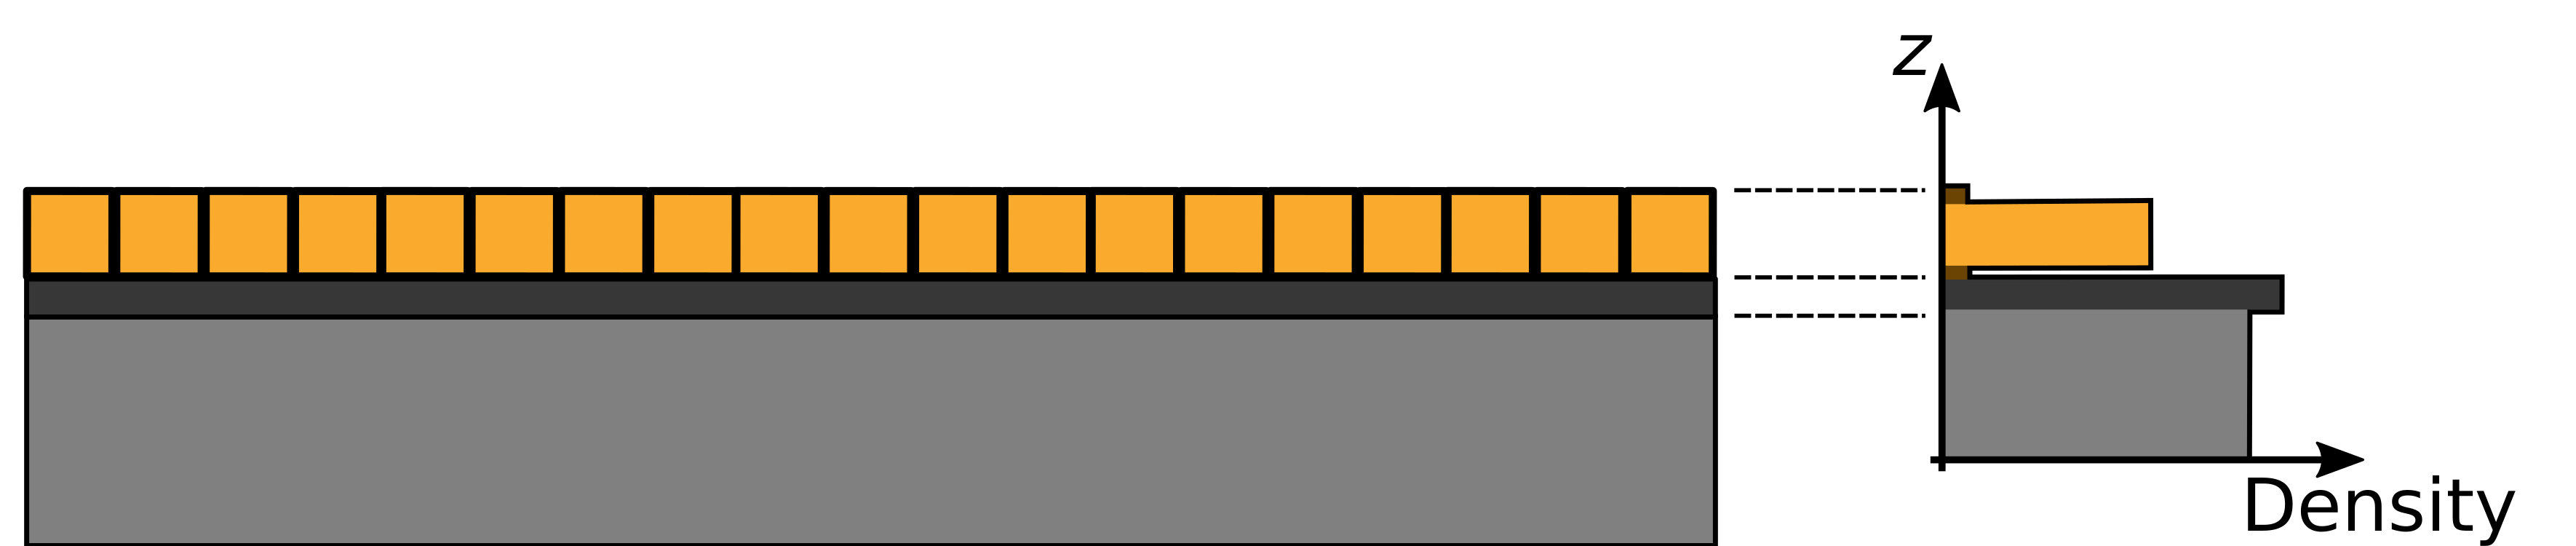
\includegraphics{monolayers_structure_verticalModel}
      \caption{\label{fig:monolayers:structure:verticalModel}Model for a square array of nanocubes depicted as cartoon of the cross-section (left) and the expected resulted shape of the vertical density structure (right). The sample can be modeled by a layered system of silicon (light gray), silicon dioxide (dark gray), oleic acid (brown) and cobalt ferrite (orange). }
    \end{figure}

    The obtained reflectivities are discussed by using the model that is schematically depicted in \reffig{fig:monolayers:structure:verticalModel}.
    The substrate is set to be silicon with a layer of silicon dioxide on top.
    The average lateral density of a square array layer is modeled by a single slab of nanocubes (NC), with oleic acid (OA) slabs around it.
    And at last, which is not depicted in \reffig{fig:monolayers:structure:verticalModel}, the interfaces are not clear cuts in the vertical plane, but have an interfacial roughness, which are included by Névot-Croce roughness factors in the model for each interface.

    In total this model has $4$ parameters to describe the thickness of the nanocubes, the two OA and the \ch{SiO2} layers and $5$ roughness parameters for the interfaces \ch{Si}/\ch{SiO2}, \ch{SiO2}/OA, OA/NC, NC/OA  and OA/air.
    Additionally it has $4$ parameters to describe the SLD of silicon, the \ch{SiO2}, the nanocubes and the OA.
    The edge length of the nanocubes has been determined by small-angle scattering experiments and is therefore fixed.
    And the scattering length densities of the materials are fixed to the literature values, where for X-rays the imaginary part of the scattering length density is included to account for absorption by cobalt ferrite.
    The used scattering length densities are tabulated in \reftab{tab:monolayers:charMethod:reflectometryScatteringLenghts}.
    For the NC layer a packing density factor $\eta$ is multiplied to the scattering length density to account for the particle spacing.
    The model totals therefore to $9$ refined parameters.

    \begin{table}[ht]
      \centering
      \caption{\label{tab:monolayers:charMethod:reflectometryScatteringLenghts}Scattering length values fixed in the calculation of the reflectivity. For XRR the electronic SLD $\rho_\mathrm{el.}$ is calculated for Cu-K$\alpha$ ($\lambda \eq 1.54 \unit{\angstrom}$) and for NR the nuclear SLD $\rho_\mathrm{nuc.}$ is used \cite{Sears_1992_Neutr, BerkeleyLab_1993_asf}.}
      \begin{tabular}{ l | c | c }
        \textbf{SLD}  & $\rho_\mathrm{el.} \, / \unit{10^{-6} \angstrom^{-2}}$ & $\rho_\mathrm{nuc.} \, / \unit{10^{-6} \angstrom^{-2}}$ \\
        \hline
        $\ch{Si}$                                 & $20.122 - 0.459 i$   & $2.079$  \\
        $\ch{SiO2}$                               & $22.724 - 0.294 i$   & $4.186$  \\
        Oleic Acid ($\ch{C18H34O2}$)              & $8.520  - 0.013 i$   & $0.078$  \\
        Ac-CoFe-C ($\ch{Co_{0.66}Fe_{2.22}O4}$)   & $39.445 - 3.663 i$   & $6.194$  \\
        Ac-CoFe-C-2 ($\ch{Co_{0.8} Fe_{2.13}O4}$) & $39.963 - 3.749 i$   & $6.135$  \\
        \hline
      \end{tabular}
    \end{table}

    The parameter values are refined by applying the Levenberg-Marquardt algorithm \cite{Marquardt_1963_Analgo}, to minimize the figure of merit $\mathrm{FOM}$, which is defined here for reflectometry as a $\chi^2$ function on the logarithmic scale
    \begin{align}
      \mathrm{FOM} \eq \sum_{q_i} \biggl( \log(I) - \log(I_\mathrm{model})\biggr)^2.
    \end{align}
    Due to the strong weight of the reflectivity in the small-$q$ range, the errorbars are ignored for the refinement to focus the algorithm on finding a model that describes the whole dynamic range properly.

    From the refined packing density, the relative particle spacing $a_{p-p}$ is estimated by assuming that the measured surface is fully covered by square lattice of nanocubes with SLD $\rho_\mathrm{NC}$ and the particle spacing is filled with oleic acid of SLD $\rho_\mathrm{OA}$ and thus
    \begin{align}
      \label{eq:monolayers:characterization:particleSpacing}
      \begin{split}
        &\eta \rho_\mathrm{NC}  \eq \frac{a^2}{a_{p-p}^2} \rho_\mathrm{NC} + \frac{a_{p-p}^2 - a^2}{a_{p-p}^2} \rho_\mathrm{OA},\\
        \Rightarrow& a_{p-p} \eq a \sqrt {\frac{\rho_\mathrm{NC} - \rho_\mathrm{OA} }{\eta \rho_\mathrm{NC} - \rho_\mathrm{OA}}}
      \end{split}
    \end{align}

    \paragraphNewLine{Grazing-Incidence Small-Angle X-ray Scattering}
      The sample ML-Ac-CoFe-C-2 has been measured by GISAXS by using the GALAXI instrument (\refsec{ch:lss:galaxi}) ($\lambda \eq 1.34 \unit{\angstrom}$).
      The incident angle was chosen to $0.15 ^\circ$ at a sample-to-detector distance of $1.733 \unit{m}$.
      An initial evaluation of the GISAXS is performed analogue to the discussion of the GISAXS detector images obtained for the samples from solvent variation in \refsec{sec:monolayers:nanoparticle:dropcastingExperiments} by fitting a Voigt function to the first order peak in the Yoneda band.
      From the fitted parameters, the lattice constant $a$, coherence length $L_\mathrm{coh.}$ and uncertainty of the nearest neighbour position $\sigma_\mathrm{n.N.}$ is estimated.

      For a more precise investigation of the grazing-incidence scattering, the BornAgain software package \cite{Burle_2018_borna} is used to simulate the two dimensional detector data by the model of nanocubes with a paracrystalline square lattice interference function.
      The edge length, it's size distribution and the scattering length density of the nanocubes are set to the values obtained from the nanoparticle characterization by small-angle scattering in \refsec{sec:monolayers:nanoparticles}.
      Similar to the vertical structure model, it is assumed the sample is a multi layer structure with a \ch{Si} substrate, a \ch{SiO2} intermediate layer and the nanocubes sit within an oleic acid layer.
      As layer thickness, the same values as in XRR and the SLD of the layers are calculated from literature using the GALAXI wavelength of $1.34 \unit{\angstrom}$ for each material respectively.
      The Gaussian broadening is included to simulate the instrumental resolution of GALAXI.
      In the simulation, it is assumed that the orientation of the lattice is on average random with respect to the beam and the probability functions of the position uncertainty in the square lattice paracrystal are assumed to be Gaussian functions.
\end{document}